\section{Moral Hazards}

\subsection{A Simple Model for a Moral Hazard}

A moral hazard occurs when capital providers cannot monitor the actions of an agent who controls funds and may extract value. For example, a \say{too-big-to-fail} bank might pursue tail-risk trades, knowing deposit insurance limits its downside. 

We analyze a canonical model of entrepreneurial effort and financing constraints, adapted from \citet{holmstrom2011inside} and summarized in \autoref{fig:fig7}.

\begin{figure}[h]
    \centering
    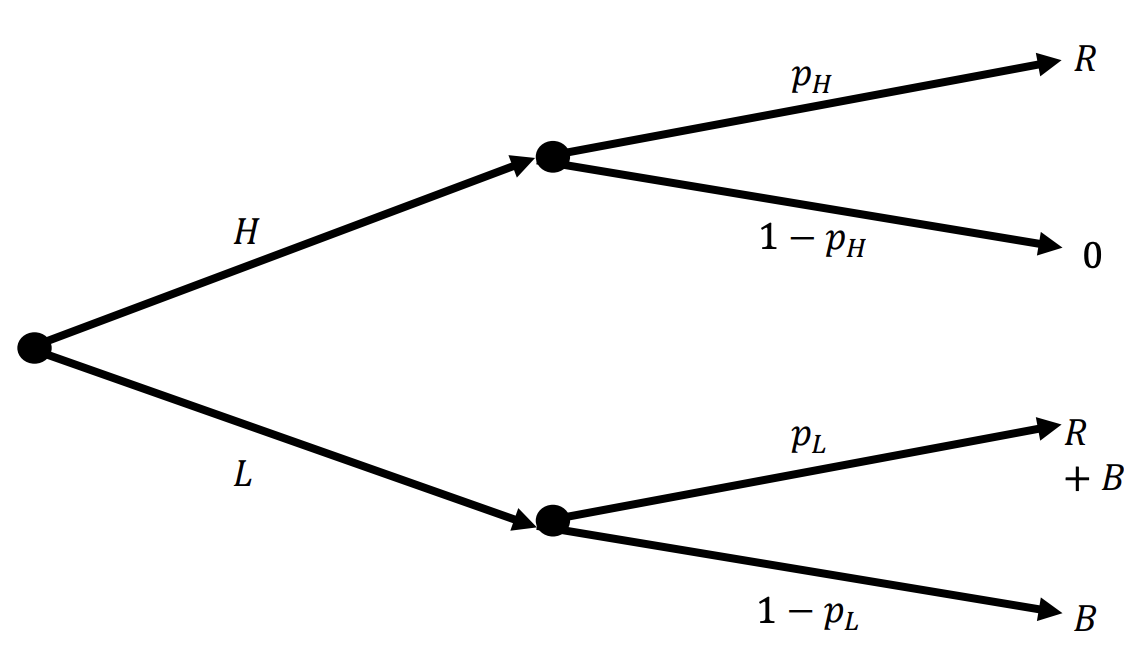
\includegraphics[width=0.75\textwidth]{fig7.png}
    \caption{Financing constraint under moral hazard}
    \label{fig:fig7}
\end{figure}

Consider a single entrepreneur who requires outside investment of $I$ to launch a project that will pay $R$ upon success but nothing upon failure. When the entrepreneur works hard (the high-effort choice), the project succeeds with probability $p_H$. Conversely, shrinking to a low-effort level lowers the success probability to $p_L$, where $p_L < p_H$ but allows the entrepreneur to get a private benefit of $B$ (i.e., perks or diverted cash) assumed to be certain. We assume the following conditions:
\begin{itemize}
    \item The project is socially efficient: $p_H R > I$
    \item Private benefit is not so large that it outweighs the high-effort surplus, due to decreasing marginal utility and how companies often succeed in creating wealth for large dispersed shareholders: $B< p_H R$
    \item Investors would still break even if the entrepreneur shirks: $I < p_L R$
\end{itemize}

The risk arises because investors cannot observe effort directly, so they must design a contract that makes high effort preferable. Let the contract promise the entrepreneur $X_s (\ge 0)$ if the project succeeds and $X_f$ if it fails. For high effort to dominate low effort, the entrepreneur's expected payoff from exerting effort must weakly exceed the payoff from shirking:
\[
p_H (R - X_s) + (1 - p_H) X_f \geq p_L (R - X_s) + (1 - p_L) X_f + B
\]

Subtracting both sides yields:
\[
X_s - X_f \geq \frac{B}{\Delta p}
\quad \text{where } \Delta p = p_H - p_L
\]


Since limited liability prevents investors from charging the entrepreneur money after a failure, we can assume $X_f = 0$. Thus, the minimum success-state payment is $X_s^{min} = \frac{B}{\Delta p}$. Note that every dollar committed to $X_s^{min}$ is a dollar that cannot be pledged to investors. Every dollar allocated to $X_s^{min}$ cuts the cash flow investors can claim; thus, the largest expected cash-flow is $p_H(R- \frac{B}{\Delta p})$.

Financing this project is only feasible if the required capital $I$ does not exceed this amount. If $I> p_H(R- \frac{B}{\Delta p})$, no contract can keep both the entrepreneur honest and allow investors to break even, so the project would die in the fund-raising stage.

Note the restrictions of the model, as it distills the distribution of returns from \autoref{fig:fig6} into binary outcomes: success or failure. Moreover, the multiple ways an entrepreneur can influence a project for better or worse are also collapsed into choices labeled “high” and “low” effort.


\subsection{How Market Regulation Can Help}
Market regulation can ease the moral‑hazard financing constraint by shrinking the entrepreneur’s private benefit $B$ or raising $\Delta p$. Rules regarding insider trading and limits on related-party transactions directly reduce $B$. Mandatory disclosure and continuous reporting improve monitoring, so low effort is more likely to be detected and prevented, raising $\Delta p$. 

Though this may seem to make things worse for the entrepreneur because a private benefit is going away, the entrepreneur would far rather receive a share of profits from a successful venture than not be able to finance a venture at all. By expanding the set of projects that attract funding and protecting outside money, well‑designed regulation is therefore Pareto‑improving: it benefits both entrepreneurs and investors through efficient capital allocation \citep{holmstrom2011inside}.

In doing so, regulation makes broad-based risk-sharing (i.e., modern equity markets) feasible at scale.